
\subsection{A Market Just Deep Enough}

The napkin was already cluttered, but Hart kept writing.

``There are about 5{,}000 hedge funds globally,'' he said, thinking aloud. ``Call it 2{,}000 
that are small-to-mid tier. The kind that can’t build their own infra stack.''

David leaned over the table.

``Assume 5\% are actively trying to expand into ML-based quant. That’s 100 funds.  
We could reasonably sell to half over five years if we build a reputation. So 50 logos?''

Hart nodded.

``Call it 10 the first year. If they pay \$250{,}000 each, that’s \$2.5 million topline.  
Think pilot licenses, integration, and support.''

David sipped his drink. ``And that’s before we license the IP or run API-based usage tiers.''

``Exactly,'' Hart said. ``If even 20\% of the target market scales usage and upgrades to \$500{,}000 per year,  
we’re looking at \$10–15 million annual run rate within 3 years.''

David tapped the napkin.

``So you frame it like this:''

The napkin was a mess — arrows, margins crowded with dollar signs, numbers scribbled into a funnel. But as David 
stared at it, something clicked.

It reminded him of how he got his first job.

Not from a polished resume — but from answering a market sizing question scrawled on the back of a flyer at a campus event.
“Size the market for enterprise AI in logistics.” No internet. No prep.

He broke it down on the spot — industry size, adoption curve, price points — drew a funnel, gave a number.
Rough. Fast. Believable.

That got him in the door.

Now here he was, years later, doing the same thing:
\begin{itemize}
    \item 2,000 funds 
    \item 5\% early adopters 
    \item 50 clients 
    \item \$250k each.
\end{itemize}

No slides. Just ink and instinct.

And for a moment, he smiled.
The math hadn’t changed.
Only the stakes had.

\medskip

\begin{figure}[H]
    \centering
    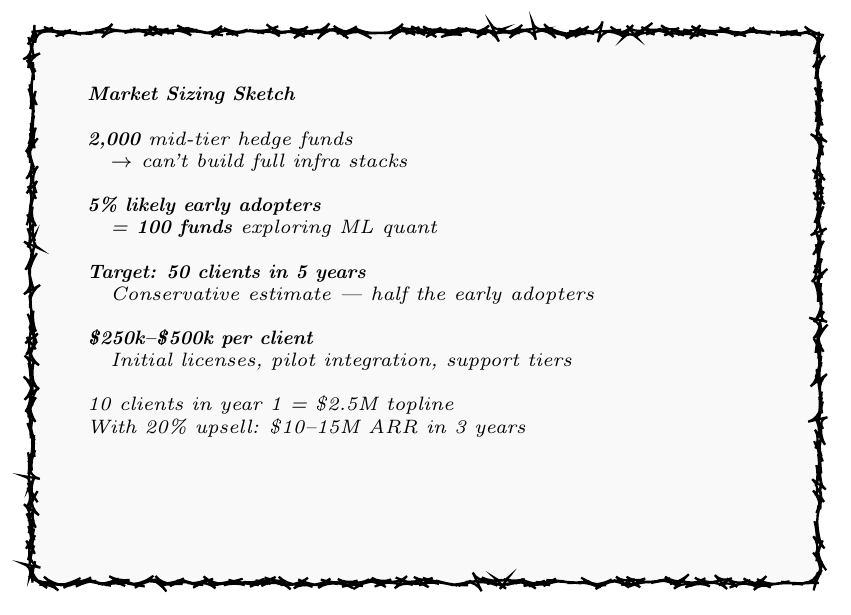
\begin{tikzpicture}[
      font=\footnotesize,
      fuzz/.style={draw=black, thick, rounded corners, fill=gray!5, decorate, decoration={random steps, segment length=2pt, amplitude=1pt}},
      txt/.style={align=left, font=\scriptsize\itshape},
    ]
  
    % Napkin box
    \node[fuzz, minimum width=10cm, minimum height=7cm, anchor=north west] (napkin) at (0,0) {};
  
    % Content inside
    \node[txt, anchor=north west] at ([xshift=0.6cm, yshift=-0.6cm]napkin.north west) {
      \textbf{Market Sizing Sketch} \\
      \\
      \textbf{2{,}000} mid-tier hedge funds \\
      \quad $\rightarrow$ can't build full infra stacks \\
      \\
      \textbf{5\% likely early adopters} \\
      \quad = \textbf{100 funds} exploring ML quant \\
      \\
      \textbf{Target: 50 clients in 5 years} \\
      \quad Conservative estimate — half the early adopters \\
      \\
      \textbf{\$250k–\$500k per client} \\
      \quad Initial licenses, pilot integration, support tiers \\
      \\
      \textit{10 clients in year 1 = \$2.5M topline} \\
      \textit{With 20\% upsell: \$10–15M ARR in 3 years}
    };
  
    \end{tikzpicture}
    \caption{Napkin Summary: Market sizing and revenue projection for ML quant infrastructure sales.}
\end{figure}

\medskip

Hart leaned back, smiling.

``Exactly. Market isn’t huge. But it’s deep. It's high trust, high margin, and high retention.  
And once the first five logos land, the rest follow.  
Because nobody wants to be the last quant fund without a real-time audit layer.''

David nodded slowly.

``And if you wrap the IP into a licensing structure, the revenue multiple goes from 5x to 12x overnight.  
TAM is maybe \$500 million globally. We don’t need it all. We just need the perception that we could take 10\%.''

Hart smirked.

``And that’s how you Fermi your way into a \$50 million valuation in the first year after deployment.''


\medskip

\begin{TechnicalSidebar}{Business Viability, Payback Period, and Why VCs Care About Speed}

    One of the most underrated metrics in early-stage venture capital isn’t TAM, burn rate, or even ARR.  
    It’s \textbf{payback period} — the time it takes for a new customer to generate enough revenue to cover their own acquisition cost (Croll \& Yoskovitz, 2013; Mullins \& Komisar, 2009).
    
    \medskip
    
    \textbf{Payback Period Formula:}
    \[
    \text{Payback Period} = \frac{\text{Customer Acquisition Cost (CAC)}}{\text{Gross Margin from Customer per Month}}
    \]
    
    \medskip
    
    If it costs \$50,000 to close a deal and that customer brings in \$25,000 per month in margin,  
    the payback period is 2 months (Mauboussin \& Callahan, 2020).
    
    \medskip
    
    \textbf{Why it matters:}
    
    \begin{itemize}
      \item Short payback = fast reinvestment cycles. A startup can recycle revenue into more growth without needing new funding.
      \item Long payback = higher risk. The startup must float costs for months (or years) before breakeven.
      \item For VC firms, short payback implies \textbf{capital efficiency} — every dollar deployed drives quicker returns (Zider, 1998).
    \end{itemize}
    
    \medskip
    
    In the case of Hart and Morales’ strategy:
  
    \medskip
    
    \begin{itemize}
      \item Each client pays \$250K to \$500K annually.
      \item The product is deployed quickly — modular, containerized, low-integration overhead.
      \item Gross margins exceed 80\%, given the IP-heavy, low-support model.
    \end{itemize}
    
    \medskip
    
    Even assuming \$50K to acquire each customer, they break even within 3 months.  
    That puts them in elite territory — where CAC is recouped before the second quarter, and LTV/CAC ratios can exceed 8x (Rao, 2011).
    
    \medskip
    
    \textbf{The VC view:}  
    This isn’t just a niche tool. It’s a high-trust, high-ticket product with low churn and fast returns.
    
    \begin{quote}
    \textit{In venture math, velocity beats volume.  
    A product that pays itself back in 90 days can be scaled   
    (even before it's perfect).}
    \end{quote}
    
\end{TechnicalSidebar}
  
